\documentclass[a4paper,10pt]{article}
\usepackage[utf8x]{inputenc}
\usepackage{graphicx}
%opening
\title{Cartesian Cut Cell Grid Generator}
\author{Bruce Duncan}

\begin{document}

\maketitle

\section{Introduction}

This software implements the Cut Cell method as described by \cite{dingram}. It
is intended to provide a computation mesh for the simulation of the flow around
solid bodies in Code\_Saturne \cite{code_saturne}.

\section{Method}

The cut cell method produces a computational mesh which is mostly cartesian
except where cartesian cells intersect the solid, where the mesh is
tetrahedral. To achieve this, the library creates a background grid of unit
cubes at each point in three dimensions. It then computes the intersection of
each of these cubes with the solid and proceeds based on the output:
\begin{itemize}
 \item If the result contains no points, then the cube is completely inside the
solid and no processing is required,
\item If the result contains only the eight points of the original cube, then
the cube is completely outside the solid and will be processed as a fluid cell,
and,
\item If the result is neither of these, the cell must be cut to fit the
boundary of the solid.
\end{itemize}

The latter case, which involves computing the tetrahedral mesh of the cut cells,
is the most interesting. For reasons which will become clear in the next
section, we decompose the resulting polyhedron of each cell into many convex
polyhedra. These polyhedra are then further decomposed into tetrahedra before
being output.

\section{Implementation}

The software uses the Computational Geometry Algorithms Library (CGAL)
\cite{cgal}, which is a C++ library which uses templates to provide different
behaviour through various number ``kernels''. It provides ``Nef\_polyhedra'', a
polyhedron whose structure is specified through a boundary representation
with a local sphere map description of vertices. A sphere map is a polyhedron of
dimension two which provides a complete representation of the boundary of the 3D
polyhedron. This representation is closed under boolean operations and we rely
on this to produce polyhedra which are not malformed.

The ``cutcell'' program is written in C++ to allow easy integration with CGAL
and the CFD General Notation System (CGNS) \cite{cgns} C library, which is well
supported by Code\_Saturne.

\section{Usage Instructions}

\begin{figure}[!tbh]
 \centering
 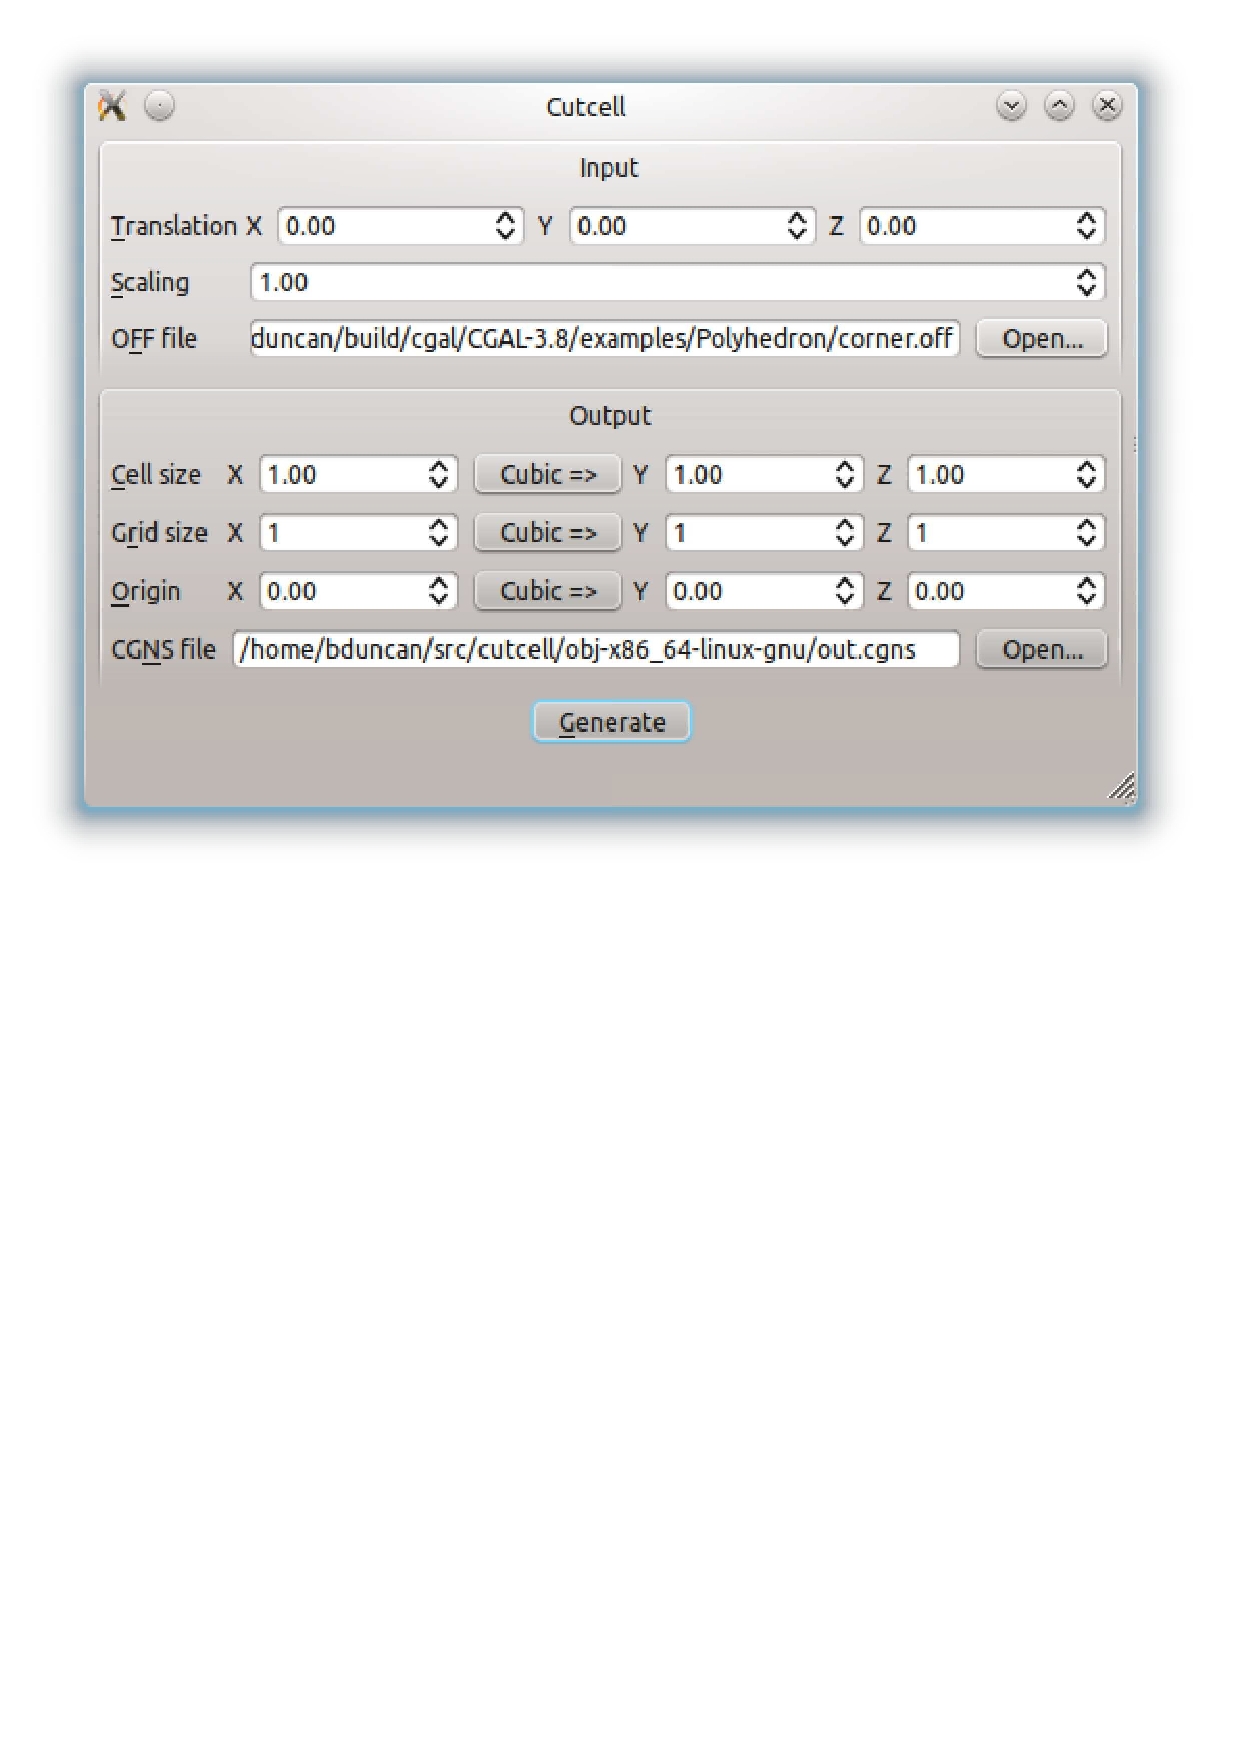
\includegraphics[keepaspectratio=true,width=\textwidth]{./cutcellgui.pdf}
 % cutcellgui.pdf: 595x842 pixel, 72dpi, 20.99x29.70 cm, bb=0 0 595 842
 \caption{The cutcell GUI}
 \label{fig:gui}
\end{figure}

The software consists of two user interfaces to the library, one Graphical User
Interface (GUI) shown in Figure~\ref{fig:gui} and one Command Line Interface
(CLI). Both allow the user to convert a polyhedral surface in Object File Format
(OFF) to a CGNS mesh. Both allow the user to specify scaling and translation
parameters for the input solid, and allow a grid size, cell size and origin to
be specified.

In using the GUI, the user is presented with default values for the position of
the input solid and the properties of the grid, these being zero or one as
appropriate. The position and size of the input solid may be specified as a
translation vector and a scale factor in three dimensions. The output CGNS grid
may have an arbitrary cell size in three dimensions, an integer number of grid
cells in each dimension and an arbitrary translation vector for the origin.

\section{Results}

\end{document}
